\documentclass[11pt, a4paper, twoside]{article}   	% use "amsart" instead of "article" for AMSLaTeX format

\usepackage{geometry}                		% See geometry.pdf to learn the layout options. There are lots.
\usepackage{pdfpages}
\usepackage{caption}
\usepackage{minted}
\usepackage[german]{babel}			% this end the next are needed for german umlaute
\usepackage[utf8]{inputenc}
\usepackage{color}
\usepackage{graphicx}
\usepackage{titlesec}
\usepackage{fancyhdr}
\usepackage{lastpage}
\usepackage{hyperref}
% http://www.artofproblemsolving.com/wiki/index.php/LaTeX:Symbols#Operators
% =============================================
% Layout & Colors
% =============================================
\geometry{
   a4paper,
   total={210mm,297mm},
   left=20mm,
   right=20mm,
   top=20mm,
   bottom=30mm
 }	

\definecolor{myred}{rgb}{0.7,0.3,0.4}
\definecolor{mygreen}{rgb}{0,0.6,0}
\definecolor{mygray}{rgb}{0.5,0.5,0.5}
\definecolor{mymauve}{rgb}{0.58,0,0.82}

\setcounter{secnumdepth}{4}


% the default java directory structure and the main packages
\newcommand{\dotNetRoot}{../source/dot-net}
\newcommand{\javaRoot}{../source/java}
\newcommand{\imagesRoot}{images}
% the default subsection headers
\newcommand{\ideaSection}{Lösungsidee}
\newcommand{\sourceSection}{Source-Code}
\newcommand{\testSection}{Tests}

% =============================================
% Code Settings
% =============================================
\newenvironment{code}{\captionsetup{type=listing}}{}
\newmintedfile[javaSourceFile]{java}{
	linenos=true, 
	frame=single, 
	breaklines=true, 
	tabsize=2,
	numbersep=5pt,
	xleftmargin=10pt,
	baselinestretch=1,
	fontsize=\footnotesize
}
\newmintinline[inlineJava]{java}{}
\newminted[javaSource]{java}{
	breaklines=true, 
	tabsize=2,
	autogobble=true,
	breakautoindent=false
}
\newmintedfile[xmlSourceFile]{xml}{
	linenos=true, 
	frame=single, 
	breaklines=true, 
	tabsize=2,
	numbersep=5pt,
	xleftmargin=10pt,
	baselinestretch=1,
	fontsize=\footnotesize
}
\newmintedfile[propertiesFile]{properties}{
	linenos=true, 
	frame=single, 
	breaklines=true, 
	tabsize=2,
	numbersep=5pt,
	xleftmargin=10pt,
	baselinestretch=1,
	fontsize=\footnotesize
}
% =============================================
% Page Style, Footers & Headers, Title
% =============================================
\title{Übung 3}
\author{Thomas Herzog}

\lhead{Übung 3}
\chead{}
\rhead{
\includegraphics[scale=0.10]{FHO_Logo_Students.jpg}}

\lfoot{S1310307011}
\cfoot{}
\rfoot{ \thepage / \pageref{LastPage} }
\renewcommand{\footrulewidth}{0.4pt}
% =============================================
% D O C U M E N T     C O N T E N T
% =============================================
\pagestyle{fancy}
\begin{document}
\setlength{\headheight}{15mm}
%\includepdf[pages={1-3}]{Swe4xA05-BB.pdf}
{\color{myred}
	\section
		{UFO (Ultimate - Festival - Organizer)}
}
Folgende Dokumentation stellt die Gesamtdokumentation der aufbauenden Übung UFO dar, die im Zuge der Realisierung iterativ über die drei Ausbaustufen hinweg erweitert wird. \\

\subsection{Ausbaustufe 1 (ADO.NET)}
Folgender Teil dokumentiert die erste Ausbaustufe der aufbauenden Übung UFO. In diesem Teil wird die Persistenz Schicht in .NET unter Hilfenahme von ADO.NET implementiert. Aufgrund der Analyse der Gesamtaufgabenstellung wurde entschieden das vorerst nur die Persistenz Schicht an sich, also INSERT, UPDATE, DELETE, der einzelnen Entitäten realisiert wird, da die Geschäftslogik erst bei der Realisierung der Administration und des Webzugriffs endgültig feststehen wird. \\\\
Im Zuge der Realisierung des Webzugriffs wird auch der Web-Service implementiert werden müssen, der die Daten der Web Applikation zur Verfügung stellt. Dieser soll die Daten bereits gefiltert und strukturiert zur Verfügung stellen, daher besteht eine gewisse Abhängigkeit zwischen dem Web-Service und der Web Applikation sowie auch der Client Administration.\\\\
Daher wird die Web-Service Implementierung die eigentliche Geschäftslogik enthalten, die 
in einer Transaktion abgearbeitet und im wesentlichen aus den logischen Prüfungen gegen die Datenbank bestehen wird. Die einzelnen Datenabfragen, die benötigt werden können einfach hinzugefügt werden.\\
Diese Geschäftslogik soll über eine REST-API zur Verfügung gestellt werden, die spezifiziert, wie mit dem System zu interagieren ist, daher stellt dieser Web-Service die Kernkomponente des Gesamtsystems dar. 

\subsubsection{Systemaufbau}
Folgend ist der Systemaufbau der Persistenz Schicht dokumentiert.\\\\
Die folgende Auflistung illustriert dir Projektstruktur der Persistenz Schicht:
\begin{enumerate}
	\item\emph{UFO.Server.Data.Api}\\
	 Dieses Projekt enthält die Spezifikation der Persistenz Schicht in Form von 	      Interfaces, abstrakten Klassen, Exceptions und den Entitäten. 
	 \item\emph{UFO.Server.Data.MySql}\\
	 Dieses Projekt enthält die MySql spezifische Implementierung der Persistenz Schicht.
	 \item\emph{UFO.Server.Test.Data.MySql}\\
	 Dieses Projekt enthält die MySql spezifischen Tests der Persistenz Schicht.
	 \item\emph{UFO.Common.Util}\\
	 Dieses Projekt enthält die Utlities für die UFO Infrastruktur in .NET, die nicht spezifisch einen Systemteil zuzuordnen ist.
\end{enumerate}
Alle .NET Systemteile werden unter dem Namensraum \emph{UFO.*} zusammengefasst.

\newpage
Die folgende Auflistung illustriert die verwendeten Technologien und Frameworks:
\begin{enumerate}
	\item\emph{MySql}\\
	Es wird eine MySql Datenbank verwendet, die Open-Source ist und eine Integration in .NET besitzt.
	\item\emph{NUNIT}\\
	Als Test-Framework wird NUNIT verwendet, da es mehr Funktionalität mitbringt als das Standard Test-Framework integriert in .NET.
	\item\emph{ADO.NET}\\
	Als Persistenz Provider wird wie gewünnscht ADO.NET und kein ORM Mapper verwendet.
\end{enumerate}

\newpage
\subsubsection{Datenbank}
Es wurde als Datenbank MySql und Moderlierungstool MySql Workbench gewählt, da diese Datenbank erstens Open-Source, zweitens eine gute .NET Integration vorhanden ist sowie drittens bereits Erfahrungen mit dieser Datenbank vorhanden waren.\\\\
Das folgende ER-Diagramm illustriert das implementierte Datenbank Schema.
\begin{figure}[h]
	\centering
	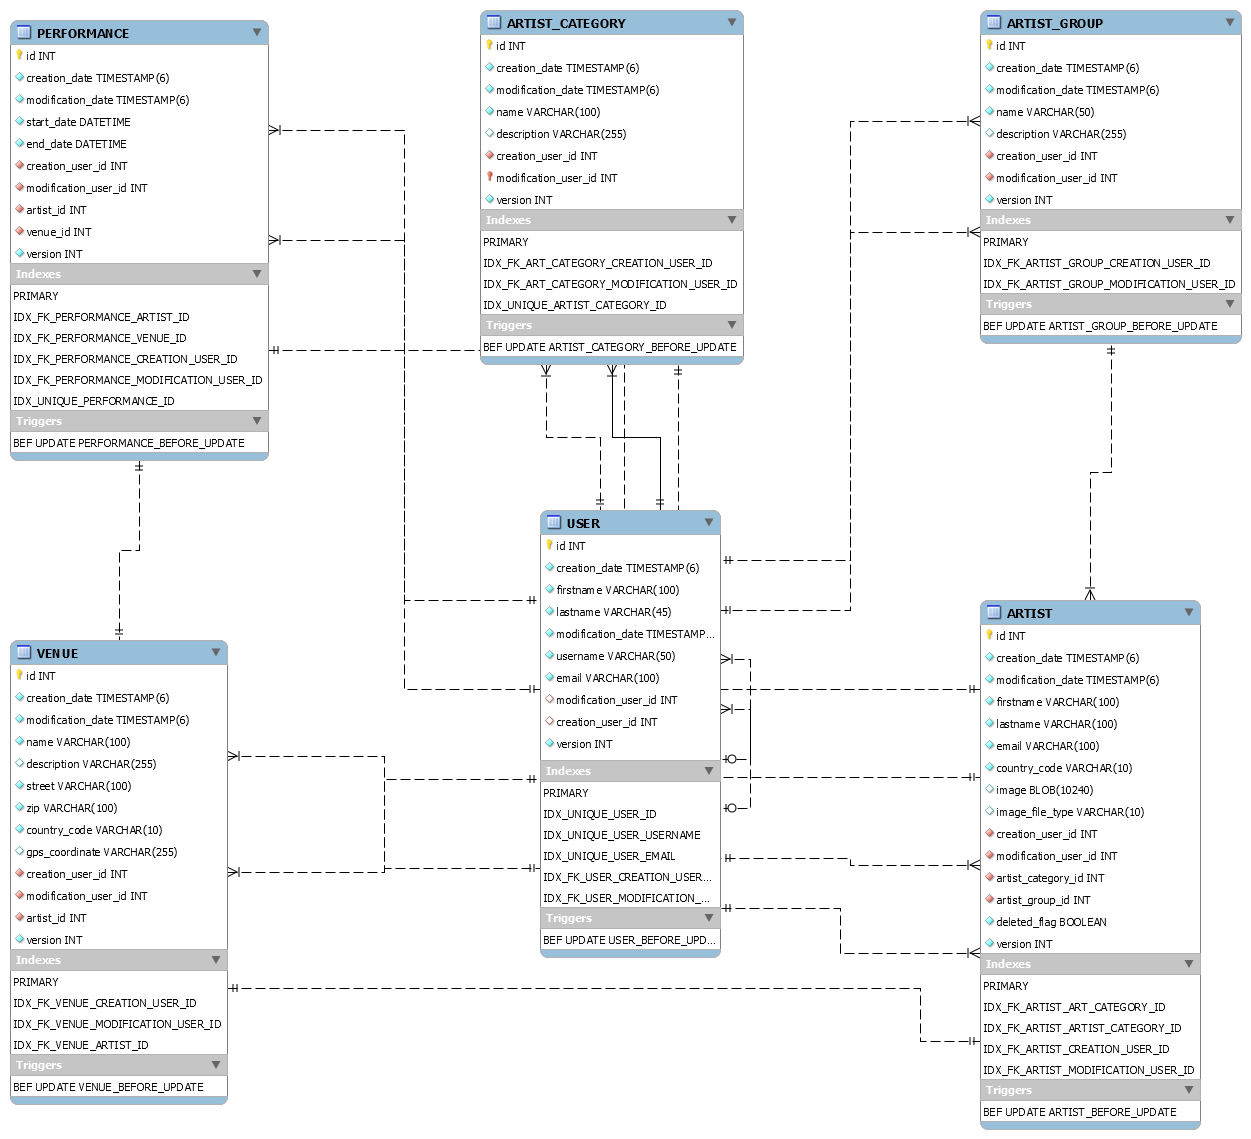
\includegraphics[scale=0.4]{\imagesRoot/er_diagram.PNG}
	\caption
	{ER-Diagramm des Schema 'UFO'}
\end{figure}
\ \\
Auf jeder Entität wurde eine Spalte für die Versionierung eingeführt (MySqlDbType.LONG), die über einen Update-Trigger bei jedem Update um eins erhöht wird sowie auch das Modifizierungsdatum. Ein ganzahliger Datentyp erschient hier mehr sinnvoll, da es hier mit Sicherheit keine Kollisionen geben kann, nicht so wie bei einem Timestamp Datentyp.\\\\
Ebenso halten alle Entitäten eine Referenz auf den Benutzer der Sie erstellt sowie zuletzt modifiziert hat. Dies dient der Nachverfolgbarkeit von Änderungen, zumindest wer zuletzt eine Änderung durchgeführt hat.

\newpage
\subsubsection{Klassenhierarchien}
Folgend ist die Struktur der Klassenhierarchien dokumentiert.

\emph{IDao}\\
Folgendes Klassendiagramm zeigt die Hierarchie des Interfaces \emph{IDao}, das der Basistyp für alle implementierten DAO Interfaces dient, da es bereits alle Basisaktionen auf eine Entität definiert.
\begin{figure}[h]
	\centering
	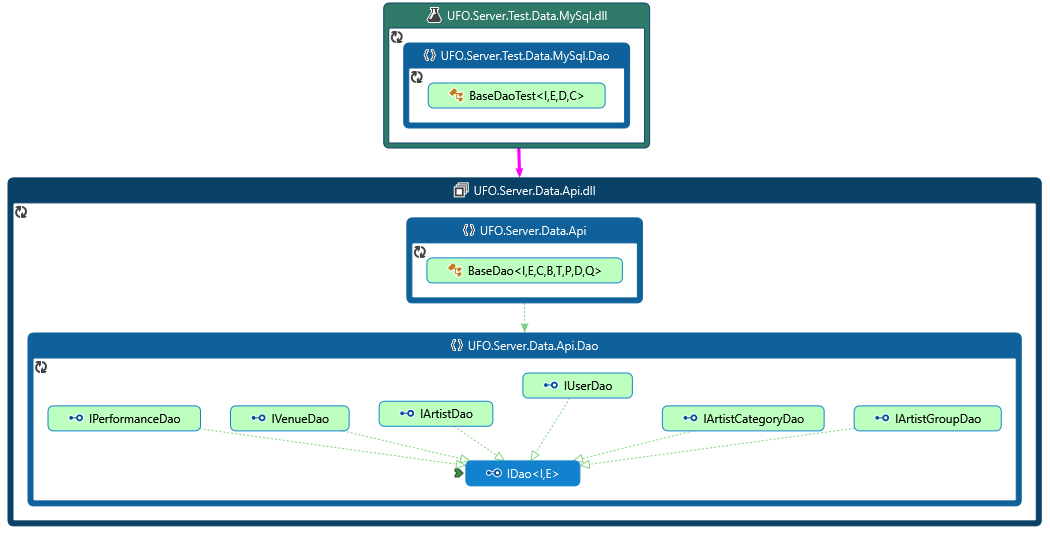
\includegraphics[scale=0.65]{\imagesRoot/idao_map.PNG}
	\caption
	{Klassenhierarchie IDao Interface}
\end{figure}
\ \\
Die Basisklasse  \emph{BaseDao} implementiert alle Methoden, die in \emph{IDao} definiert wurden für alle implementieren Entitäten sofern sie \emph{IEntity} implementieren. Dieser generische und abstrakte Ansatz erlaubt es dass die Basisfunktionalität eines DAOs nur einmal für alle Entitätstypen, die \emph{IEntity} implementieren, implementiert werden musste.

\newpage
\emph{IEntity}\\
Folgendes Klassendiagramm illustriert die Klassenhierarchie des Interfaces \emph{IEntity}, welches den Basistyp für alle Entitäten darstellt.
\begin{figure}[h]
	\centering
	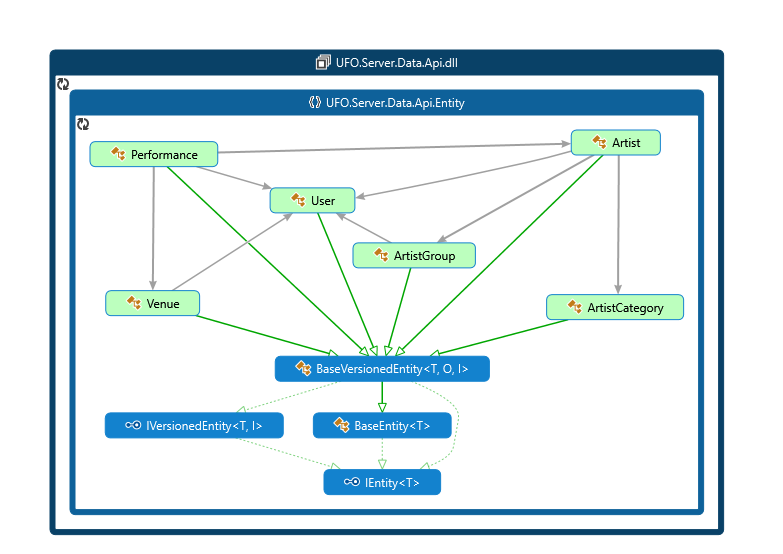
\includegraphics[scale=0.65]{\imagesRoot/ientity_map.PNG}
	\caption
	{Klassenhierarchie IEntity Interface}
\end{figure}
\ \\
Es wurden Basisentitäten eingeführt, welche eine Basisstruktur definieren dies sich Entitäten unterwerfen müssen wenn sie von diesen Klassen ableiten. Somit wird eine konsistente Struktur der Entitäten bzw. deren Tabellenrepräsentation gewährleistet.

\newpage 
\emph{IEntityHelper}\\
Folgendes Klassendiagramm illustriert die Klassenhierarchie des Interfaces \emph{IEntityHelper}.
\emph{IEntity}, welches den Basistyp für alle Entitäten darstellt.
\begin{figure}[h]
	\centering
	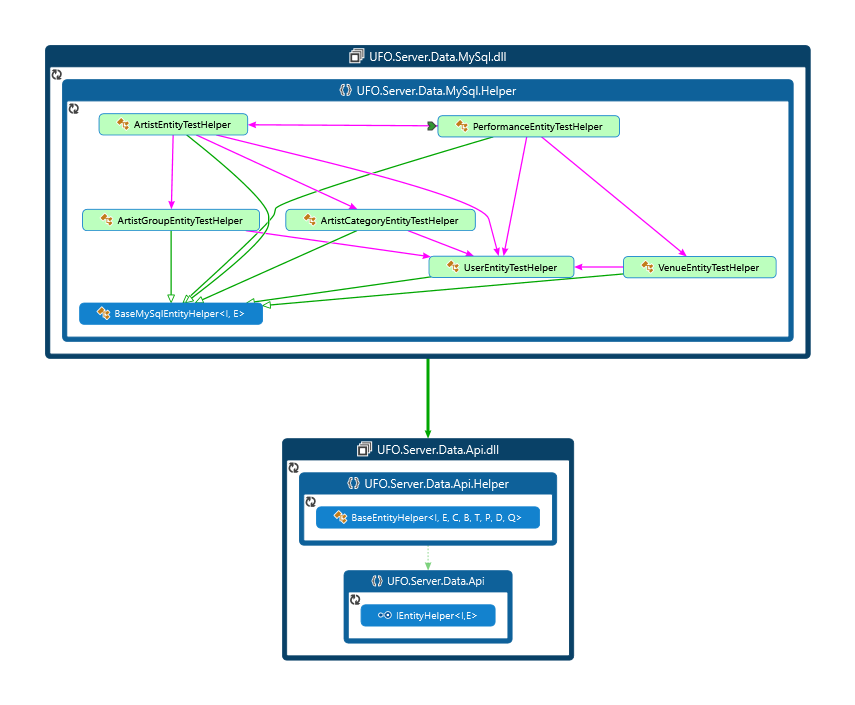
\includegraphics[scale=0.52]{\imagesRoot/ientityhelper_map.PNG}
	\caption
	{Klassenhierarchie IEntityHelper Interface}
\end{figure}
\ \\
Dieses Interface und dessen Implementierungen diesen als Hilfestellung für Test und die Generierung von Testdaten über die Entitäten Modelle. Würde hier die unabhängige Persistenz Logik in \emph{BaseEntityHelper} auh noch ausgelagert werden do könnte man diese Hiflsklassen ebenfalls in das Projekt \emph{UFO.Server.Data.Api} überführt werden, da hier nur in der Persistenz Logik die Abhängigkeiten zum Persistenz Provider enthalten sind. Diese Hilfklassen entstanden aufgrund der generischen Testklasse \emph{BaseDaoTest}, die die Entitäten nicht erzeugen kann und daher diese außerhalb geschehen muss.

\end{document}  